\chapter{TCP数据流和与窗口管理}

\section{引言}
第13章介绍了 TCP 连接的建立和终止,第14章则讨论了TCP 怎样利用丢失数据的重传来保证传输可靠性。下面我们探讨TCP的动态数据传输,首先关注交互式连接,接着介
绍流量控制以及窗口管理规程。批量数据传输中的拥塞控制策略(参见第16章)也包含了相应的窗口管理机制。

“交互式”TCP连接是指,该连接需要在客户端和服务器之间传输用户输入信息,如按键操作、短消息、操作杆或鼠标的动作等。如果采用较小的报文段来承载这些用户信息,那
么传输协议需要耗费很高的代价,因为每个交换分组中包含的有效负载字节较少。反之,报文段较大则会引入更大的延时,对延迟敏感类应用(如在线游戏、协同工具等)造成负面影
响。因此我们需要权衡相关因素,找到折中方法。

在讨论交互式通信的相关问题后,会介绍 TCP流量控制机制。它通过动态调节窗口大小来控制发送端的操作,确保接收端不会溢出。这个方法主要用于批量数据传输(即非交互
式通信),但对交互式应用也同样有效。在第16章我们会看到,流量控制的思想也可以扩展应用于其他问题,不仅可以保护接收端免于溢出,还可处理中间传输网络的拥塞问题。
\section{交互式通信}

在一定时间内,互联网的不同部分传输的网络流量(通常以字节或包来计算)也存在相当大的差异。例如,局域网与广域网以及不同网站之间的流量都会有所不同。TCP 流量研究
表明,通常90\%或者更多的 TCP报文段都包含大批量数据(如Web、文件共享、电子邮件、备份),其余部分则包含交互式数据(如远程登录、网络游戏)。批量数据段通常较大(1500
字节或更大),而交互式数据段则会比较小(几十字节的用户数据)。

对于使用相同协议以及封包格式的数据,TCP都会处理,但执行的算法有所不同。在本节中我们会讨论 TCP 如何传输交互式数据,以 ssh(安全外壳)应用为例。安全外壳协议
\href{https://www.rfc-editor.org/rfc/rfc4251}{[RFC4251]}是具备较强安全性(基于密码学的加密和认证)的远程登录协议。它已经基本取代了早期的 UNIX tlogin 和 Telnet,因为这些远程登录服务都存在安全隐患。

通过对ssh的探讨,我们会了解延时确认是怎样工作的,以及 Nagle 算法怎样实现减少广域网中较小包的数目。同样的算法也可以用于其他远程登录应用,如 Telnet、rlogin 和微
软终端服务。

对一个 ssh 连接,观察当我们输人一个交互命令后的数据流。客户端获取用户输入信息,然后将其传给服务器端。服务器对命令进行解释并生成响应返回给客户端。客户端对其
传输数据加密,意味着用户输入的信息在通过连接传送前已经进行了加密(参见第18章)。即使传输数据被被获,窃听者也很难获得用户输入信息的明文。客户端支持多种加密算法
和认证方法。它也支持一些新的特性,如隧道技术实现对其他协议的封装(参见第3章及\href{https://www.rfc-editor.org/rfc/rfc4254}{[RFC4254]})。

许多 TCP/IP 的初学者会惊奇地发现,每个交互按键通常都会生成一个单独的数据包。也就是说,每个按键是独立传输的(每次一个字符而非每次一行)。另外,ssh 会在远程系统
(服务器端)调用一个 shell(命令解释器),对客户端的输人字符做出回显。因此,每个输人的字符会生成4个 TCP数据段:客户端的交互击键输人、服务器端对击键的确认、服务器端
生成的回显、客户端对该回显的确认(参见图15-1a)。

通常,第2和第3段可以合并,如图15-1b所示,可将对击键的确认与回显一并传送。下一节会介绍这种方法(称力捎带延时璃认)。

a)对一次交互击键的远程回显,一种可行的方法是将对击键的确认与回显包各自独立发送。b)典型 TCP 则将两者结合传输

我们以 ssh 为例的原因在于,对从客户端到服务器键人的每个字符都会生成一个独立的包。然而,若用户的输入速度较快,每个包可能包含多个字符。图15-2显示了在ssh 连接至
Linux 服务器中输入 date 命令,利用 Wireshark 获得的数据流。

\begin{figure}[!htb]
    \centering
	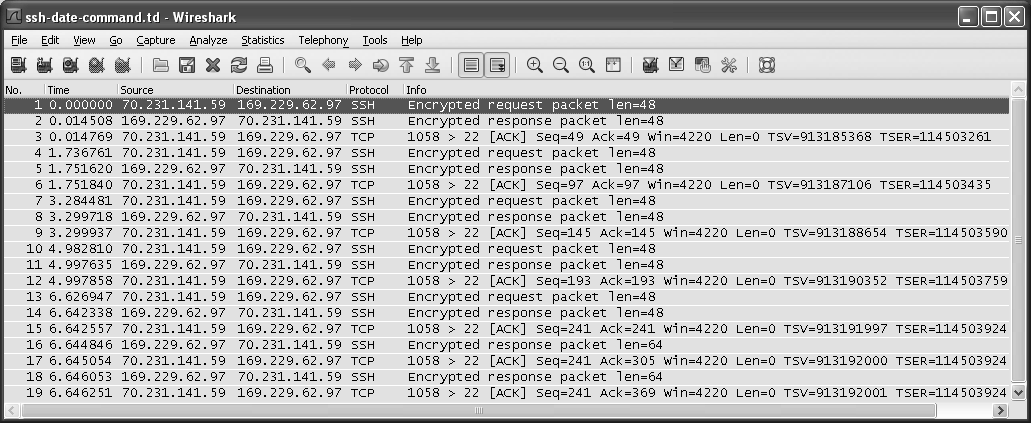
\includegraphics[width=0.7\textwidth]{imgs/15/15-2.png}
	\caption{变得更为密集。Linux 避免 RTO 设置过小就是防止这种情况的发生。标准方法在样本 78 和191 出现潜在问题}
\end{figure}

如图15-2所示,包1包含了客户端到服务器端的命令字符d。包2为对字符d的确认和回显(如图15-] 中将两段结合传送)。包3为对国显字符d的确认。同理,包4~6对应字
符日,包7-9对应字符1,包10~12对应字符e。包13~15 则对应回车键。在包3+6~7、9~10和12~13 之间的时间差为人工输入每个字符的延迟,这里特意设置得较长
(约1.5秒)。

注意到包16~19与前面的包稍有差异,包长度从48字节变为64字节。包16包含了服务器端对 date 命令的输出。这64 字节的数据是对下面28个明文(未加密)字符的加密
结果:
\begin{verbatim}
    Wed Dec 28 22:47:16 PST 2005
\end{verbatim}
加上最后的回车和换行符。下一个从服务器端发送至客户端的包(包18)包含了服务器主机对客户的命令提示符:Linux\%。包19为对该数据的确认。

图15-3描述与图15-2相同的传输情况,只是细化了 TCP 层的信息,可以更清晰地看到TCP 怎样进行确认以及 ssh 使用的包大小。包1(包含字符d)的相对序列号从0开始。包2
是对图中包1的确认,ACK 号设为48,为上次成功接收字节的序列号加1。包2也包含了服务器至客户端的对d字符的回显,字节序列号为0。包3为客户端对该回显的确认,ACK
号设为 48。可以看到,该连接包含了两个序列号流个是从客户端至服务器,另一个为相反方向。在介绍窗口通告时将会详细讨论这一问题。

\begin{figure}[!htb]
    \centering
	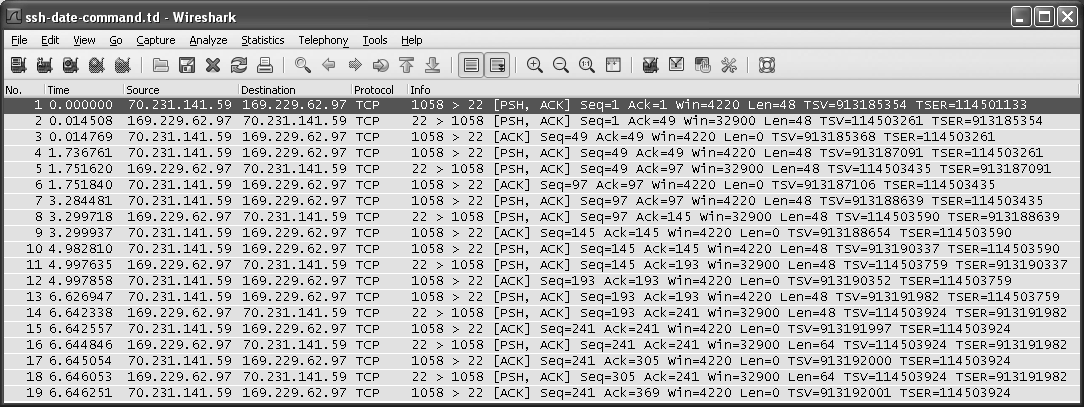
\includegraphics[width=0.7\textwidth]{imgs/15/15-3.png}
	\caption{与图 15-2相同,只是这里禁用了 ssh 的协议解码,因此可以看到 TCP 序列号信息。注意到除了最后两个包外,其他包都为48字节,该长度与 ssh 使用的加密算法有关(参见第18章)}
\end{figure}

另外我们也发现,每个带数据(长度不为0)的包都将PSH置位。之前提到过,该标志位通常表示发送端缓存为空。也就是说,当PSH 置位的数据包发送完成后,发送端没有其
他数据包需要传输。

\section{延时确认}
在许多情况下,TCP 并不对每个到来的数据包都返回 ACK,利用TCP 的累积ACK 字段(参见第12 章)就能实现该功能。累积确认可以允许 TCP 延迟一段时间发送ACK,以便
将 ACK 和相同方向上需要传的数据结合发送。这种捎带传输的方法经常用于批量数据传输。显然,TCP 不能任意时长地延迟ACK;否则对方会误认为数据丢失而出现不必要的重传。

\begin{tcolorbox}
    主机需求 RFC \href{https://www.rfc-editor.org/rfc/rfc1122}{[RFC1122]}指出,TCP 实现 ACK 延迟的时延应小于 500ms。实践中时延最大取 200ms。
\end{tcolorbox}

采用延时 ACK的方法会减少ACK 传输数目,可以一定程度地减轻网络负载。对于批量数据传输通常为2:1的比例。基于不同的主机操作系统,延迟发送ACK 的最大时延可以
动态配置。Linux 使用了一种动态调节算法,可以在每个报文段返回一个ACK(称次“快速确认”模式)与传统延时ACK 模式间相互切换。Mac OS X 中,可以改变系统变量 
\verb|net.inet.top.delayed_ack| 值来设置延时 ACK。可选值如下:禁用延时(设为0),始终延时(设为1),每隔一个包回复一个 ACK(设为2),自动检测确认时间(设次3)。默认值为3。最新的
Windows 版本中,注册表项
\begin{verbatim}
    HKLM\SYSTEM\CurrentControlSet\Services\Tcpip\Parameters\Interfaces\IG
\end{verbatim}
中,每个接口的全局唯一标识(GUID)都不同(IG 表示被引用的特定网络接口的GUID)。TepAckFrequency 值(需要被添加)可以设为0~255,默认为2。它代表延时 ACK 计时器
超时前在传的ACK 数目。将其设为1表明对每个收到的报文段都生成相应的ACK。ACK 计时器值可以通过 TopDelAckTicks注册表项控制。该值可设为2~6,默认为2。它以百毫秒
为单位,表明在发送延时ACK 前要等待百毫秒数。

之前提到过,通常 TCP 在某些情况下使用延时 ACK 的方法,但时延不会很长。在第16章中大量采用了延时 ACK 的方法,我们将会看到 TCP怎样在处理批量数据的大数据包传输
中实现拥塞控制。在小数据包传输中,如交互式应用,需要采用另外的算法。将该算法与延时 ACK 结合使用,如果处理不好,反而会导致性能降低。下面我们详细讨论该算法。

\section{Nagle 算法}
从前面的小节中可以知道,在ssh 连接中,通常单次击键就会引发数据流的传输。如果使用 IPv4,一次按键会生成约88字节大小的TCP/IPv4包(使用加密和认证):20字节的
『头部,20字节的TCP 头部(假设没有选项),数据部分为48字节。这些小包(称为微型报(tinygram))会造成相当高的网络传输代价。也就是说,与包的其他部分相比,有效的应
用数据所占比例甚微。该问题对于局域网不会有很大影响,因为大部分局域网不存在拥塞,而且这些包无须传输很远。然而对于广域网来说则会加重拥塞,严重影响网络性能。John
Nagle 在\href{https://www.rfc-editor.org/rfc/rfc0896}{[RFC0896]}中提出了一种简单有效的解决方法,现在称其为 Nagle 算法。下面首先介绍该算法是怎样运行的,接着我们会讨论结合延时 ACK 方法使用时可能出现的一些缺陷
和问题。

Nagle算法要求,当一个 TCP 连接中有在传数据(即那些已发送但还未经确认的数据),小的报文段(长度小于 SMSS)就不能被发送,直到所有的在传数据都收到ACK。并且,在
收到ACK 后,TCP 需要收集这些小数据,将其整合到一个报文段中发送。这种方法迫使TCP 遵循停等(stop-and-wait)规程—只有等接收到所有在传数据的ACK 后才能继续发
送。该算法的精妙之处在于它实现了自时钟(self-clocking)控制:ACK 返回越快,数据传输也越快。在相对高延迟的广域网中,更需要减少微型报的数目,该算法使得单位时间内发
送的报文段数目更少。也就是说,RTT 控制着发包速率。

从图15-3中可以看到,单个字节的发送、确认以及回显的RTT较小(15ms 以下)。为更快地生成数据,我们需要每秘钟输入60个字符以上。这意味着,当两台主机之间以很小
的 RTT传输数据时,例如在同一个局域网中,我们将很难看到该算法的显著效果。

为了显示 Nagle算法的效果,我们比较分析某个 TCP 应用使用和禁用该算法的行为。我们对一个 ssh 版本的客户端做了一定的修改。利用一个 RTT相对较大(约190ms)的连接,
就可以看出区别。首先观察禁用 Nagle 算法(ssh 默认)的情况,如图15-4所示。
\begin{figure}[!htb]
    \centering
	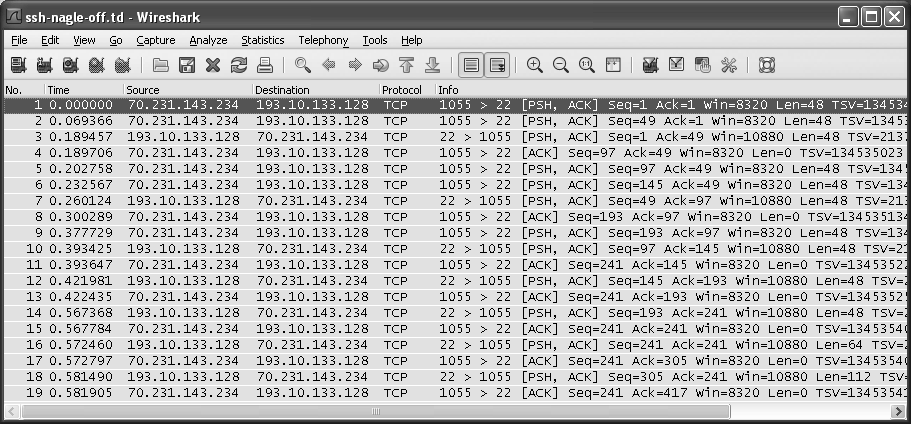
\includegraphics[width=0.7\textwidth]{imgs/15/15-4.png}
	\caption{ssh分析文件显示该TCP 连接RTT约为190ms。Nagle 算法被禁用。数据和ACK结合传输,19 个包传输持续了 0.58s。许多包相对较小(48字节的用户数据)。
    纯ACK(不包含数据的报文段)表明服务器端的输出命令已被客户端接收处理}
\end{figure}

图15-4中显示的传输是在初始的认证完成以后、登录会话开始时记录的。这时输入date 命令,我们看到共捕获到了19个包,整个传输过程持续了 0.58S。共有5个 ssh 请求包,
7个ssh 应答包,以及7个 TCP 层的纯 ACK 包(不包含数据)。下面我们将在使用Nagle算法的情况下重复探测这一过程(即在相似的网络环境下),可以得到图15-5。

RTT为190ms并启用 Nagle算法的 TCP连接的ssh传输情况。请求和响应传输规律,紧密一致。整个传输过程持续了 0.80s,共有11个包

可以看到图 15-5中的包数目要少于图15-4(少了8个)。另外一个明显的差异是,请求和响应包随时间分布呈一定的规律性。回想一下 Nagle 算法的原理,它迫使 TCP 遵循停等行
为模式,因此TCP 发送端只有在接收到全部 ACK 后才能继续发送。观察每组请求/ 响应的传输时刻—0.0、0.19、0.38以及0.57,我们可以发现它们遵循一定的模式:每两个间隔为
190ms,恰为连接的RTT。每发送一组请求和响应包需要等待一个 RTT,这就加长了整个传输过程(需要0.80s而非前面的0.58s)。Nagle 算法做出了一种折中:传输的包数目更少而长
度更大,但同时传输时延也更长。从图15-6中可以更清晰地看出差别。

图15-6显示了Nagle 算法的停等行为。左侧显示双向传输,而右侧使用 Nagle 算法,使得在任一给定时刻,只有一个方向保持传输状态。
% \begin{figure}[!htb]
%     \centering
% 	\includegraphics[width=0.7\textwidth]{imgs/15/15-6.png}
% 	\caption{比较相似环境下使用 Nagle算法与否的TCP连接情况。在启用 Nagle 算法的情况下,在任一时刻最多只有一个包在传。这样可以减少小包数目,但同时也增大了传输时延}
% \end{figure}

\subsection{延时 ACK 与 Nagle 算法结合}
若将延时ACK与Nagle 算法直接结合使用,得到的效果可能不尽如人意。考虑如下情形,客户端使用延时 ACK 方法发送一个对服务器的请求,而服务器
端的响应数据并不适合在同一个包中传输(参见图 15-7)。

从图中可以看到,在接收到来自服务器端的两个包以后,客户端并不立即发送 ACK,而是处于等待状态,希望有数据一同捎带发送。通常情况下,TCP
在接收到两个全长的数据包后就应返回一个ACK,但这里并非如此。在服务器端,由于使用了 Nagle 算法,直到收到ACK 前都不能发送新数据,因为任一
时刻只允许至多一个包在传。因此延时
ACK 与Nagle 算法的结合导致了某种程度的死锁(两端互相等待对方做出行动)[MMSV99][MMO1]。幸运的是,这种死锁并不是永久的,在延时 ACK 计时器超时后死锁会解除。客户
端即使仍然没有要发送的数据也无需再等待,而可以只发送ACK 给服务器。然而,在死锁期间整个传输连接处于空闲状态,使性能变差。在某些情况下,如这里的 ssh 传输,可以禁
用 Nagle 算法。

\subsection{禁用 Nagle 算法}
从前面的例子可以看到,在有些情况下并不适用Nagle 算法。典型的包括那些要求时延尽量小的应用,如远程控制中鼠标或按键操作需要及时送达以得到快捷的反馈。另一个例子
是多人网络游戏,人物的动作需要及时地传送以确保不影响游戏进程(也不致影响其他玩家的动作)。

禁用 Nagle 算法有多种方式,主机需求 RFC\href{https://www.rfc-editor.org/rfc/rfc1122}{[RFC1122]}列出了相关方法。若某个应用使用Berkeley 套接字 API,可以设置 \verb|TCP_NODBLAY| 选项。另外,也可以在整个系统中禁用
该算法。在 Windows 系统中,使用如下的注册表项:
\begin{verbatim}
    HKLM\ SOFTWARE \Microsoft \MSMQ \Parameters\ TCPNoDelay
\end{verbatim}
这个双字节类型的值必须由用户添加,应将其设为1。为使更改生效,消息队列也需要重新设置。

\section{流量控制与窗口管理}
回顾一下第12章中提到过,可以采用可变滑动窗口来实现流量控制。如图15-8所示,TCP 客户端和服务器交互作用,互相提供数据流的相关信息,包括报文段序列号、ACK号
和窗口大小(即接收端的可用空间)。

每个 TCP 连接都是双向的。数据传输方向的另一端会返回ACK 及其窗口通告信息。反向亦然

图15-8 中两个大的箭头表示数据流方向(TCP报文段的传输方向)。每个 TCP 都是双向连接,这里用两个箭头表示,一个是客户端至服务器方向(C一S),另一个为服务器至客户
端方向(S-C)。每个报文段包含 ACK 和窗口信息,可能还有用户数据。根据数据流传输方向的不同,将 TCP 头部中的字段标记上阴影。例如,在C一S方向的数据流为下方箭头
的报文段,但是对该数据的 ACK 和窗口信息却在上方简头指示的报文段中。每个TCP报文段(除了连接建立之初的包交换)都包含一个有效的序列号字段、一个 ACK 号或确认字段,
以及一个窗口大小字段(包含窗口通告信息)。

在前面的ssh 示例中,我们看到的窗口通告都是固定的,有8320字节、4220字节,还有32900字节。这些数值表示发送该窗口信息的通信方为即将到来的新数据预留的存储空
间。当TCP 应用程序空闲时,就会排队处理这些数据,致使窗口大小字段保持不变。当系统处理速度较慢,或者程序忙于执行其他操作,到来的数据返回ACK 后,就需要排队等待
被读取或“消耗”。若这种排队状况持续,新数据的可用存储空间就会减小,窗口大小值也随之减小。最终,若应用程序一直不处理这些数据,TCP必须采取策略使得发送端完全
停止新数据的发送,因为可能没有空间来存储新数据。此时就可以将窗口通告设为0(没有空间)。

每个 TCP 头部的窗口大小字段表明接收端可用缓存空间的大小,以字节为单位。该字段长度为16位,但窗口缩放选项可用大于65 535的值(参见第13章)。报文段发送方在相反
方向上可接受的最大序列号值为 TCP 头部中 ACK 号和窗口大小字段之和(保持单位一致)。

\subsection{滑动窗口}
TCP连接的每一端都可收发数据。连接的收发数据量是通过一组窗口结构(windowstructure)来维护的。每个 TCP活动连接的两端都维护一个发送窗口结构(send window
structure)和接收窗口结构(receive window structure)。这些结构与第12 章中描述的概念窗口结构类似,这里我们将详细讨论。图15-9显示了一个假设的TCP 发送窗口结构。

TCP 发送端滑动窗口结构记录了已确认、在传以及还未传的数据的序列号。提供窗口的大小是由接收端返回的 ACK 中的窗口大小字段控制的

TCP 以字节(而非包)为单位维护其窗口结构。在图15-9中,我们已标号为2~11字节。由接收端通告的窗口称为提供窗口(offered Window),包含4~9字节。接收端已成功
确认包括第3字节在内的之前的数据,并通告了一个6字节大小的窗口。回顾第12章,窗口大小字段相对 ACK 号有一个字节的偏移量。发送端计算其可用窗口,即它可以立即发送
的教据量。可用窗口计算值力提供窗口大小破去在传(已发送但本得到确认)的数据值。变量SND.UNA 和SND.WND 分别记录窗口左边界和提供窗口值。SND.NXT 则记录下次发送
的数据序列号,因此可用窗口值等于(SND.UNA + SND.WND -SND.NXT)。

随着时间的推移,当接收端确认数据,滑动窗口也随之右移。窗口两端的相对运动使得窗口增大或减小。可用三个术语来描述窗口左右边界的运动:
\begin{enumerate}
    \item 关闭(close),即窗口左边界右移。当已发送数据得到 ACK 确认时,窗口会减小。
    \item 打开(open),即窗口右边界右移,使得可发送数据量增大。当已确认数据得到处理,接收端可用缓存变大,窗口也随之变大。
    \item .收缩(shrink),即窗口右边界左移。主机需求 RFC\href{https://www.rfc-editor.org/rfc/rfc1122}{[RFC1122]}并不支持这一做法,但TCP必须能处理这一问题。15.5.3 节的糊涂窗口综合征中举了一个例子,一端试图将右边界左移使窗口收缩,但没有成功。
\end{enumerate}

每个TCP报文段都包含ACK 号和窗口通告信息,TCP发送端可以据此调节窗口结构。窗口左边界不能左移,因为它控制的是已确认的ACK 号,具有累积性,不能返回。当
得到的ACK 号增大而窗口大小保持不变时(通常如此),我们就说窗口向前“滑动”。若随着ACK 号增大窗口却减小,则左右边界距离减小。当左右边界相等时,称之为零窗口。此
时发送端不能再发送新数据。这种情况下,TCP 发送端开始探测(probe)对方窗口(参见15.5.2节),伺机增大提供窗口。

接收端也维护一个窗口结构,但比发送端窗口简单。该窗口结构记录了已接收并确认的数据,以及它能够接收的最大序列号。该窗口可以保证其接收数据的正确性。特别是,接收
端希望避免存储重复的已接收和确认的数据,以及避免存储不应接收的数据(超过发送方右窗口边界的数据)。图15-10描述了接收窗口结构。

TCP接收端滑动窗口结构帮助了解其下次应接收的数据序列号。若接收到的数据序列号在窗口内,则可以存储,否则丢弃

与发送端窗口一样,该窗口结构也包含一个左边界和右边界,但窗口内的字节(图中的4 ~9字节)并没有区分。对接收端来说,到达序列号小于左窗口边界(称 RCV.NXT),被
认为是重复数据而丢弃,超过右边界(RCV.WND + RCV.NXT)的则超出处理范围,也被丢弃。注意到由于 TCP 的累积 ACK 结构,只有当到达数据序列号等于左边界时,数据才不会
被丢奔,窗口才能向前滑动。对选择确认 TCP 来说,使用SACK 选项,窗口内的其他报文段也可以被接收确认,但只有在接收到等于左边界的序列号数据时,窗口才能前移(SACK
的更多细节可以参见第14章)。

\subsection{零窗口与 TCP 持续计时器}

我们了解到,TCP 是通过接收端的通告窗口来实现流量控制的。通告窗口指示了接收端可接收的数据量。当窗口值变为0时,可以有效阻止发送端继续发送,直到窗口大小恢复
为非零值。当接收端重新获得可用空间时,会给发送端传输一个窗口更新(window update),告知其可继续发送数据。这样的窗口更新通常都不包含数据(为“纯ACK”),不能保证其传
输的可靠性。因此 TCP 必须有相应措施能处理这类丟包。

如果一个包含窗口更新的 ACK 丢失,通信双方就会一直处于等待状态:接收方等待接收数据(已将窗口设为非零值),发送方等待收到窗口更新告知其可继续发送。为防止这种死
锁的发生,发送端会采用一个持续计时器间歇性地查询接收端,看其窗口是否已增长。持续计时器会触发窗口探测(window probe)的传输,强制要求接收端返回 ACK(其中包含了窗
口大小字段)。主机需求 RFC \href{https://www.rfc-editor.org/rfc/rfc1122}{[RFC1122]} 建议在一个 RTO 之后发送第一个窗口探测,随后以指数时间间隔发送(与第14章讨论过的 Kam 算法中的“第二部分”类似)。

窗口探测包含一个字节的数据,采用TCP 可靠传输(丢失重传),因此可以避免由窗口更新丢失导致的死锁。当TCP持续计时器超时,就会触发窗口探测的发送。其中包含的一
个字节的数据是否能被接收,取决于接收端的可用缓存空间大小。与TCP 重传计时器(参见第14章)类似,可以采用指数时间退避来计算持续计时器的超时。而不同之处在于,通常
TCP 不会停止发送窗口探测,由此可能会放弃执行重传操作。这种情况可能导致某种程度的资源耗尽,我们将在15.7节中讨论这一问题。

\subsubsection{例子}

为了说明 TCP的动态窗口调节和流量控制机制,我们建立了一个 TCP 连接,并使其在处理接收到的数据之前暂停接收。本实验采用了 Mac OS X 10.6发送端和 Windows 7 接收
端。在接收端运行带-P 选项的 sock 程序:
\begin{verbatim}
    C: \> sock -1 -s -P 20 6666
\end{verbatim}
该命令使得接收端在处理接收到的数据前暂停 20s。这样就导致接收端的通告窗口在125号包处开始关闭,如图 15-11 所示。
\begin{figure}[!htb]
    \centering
	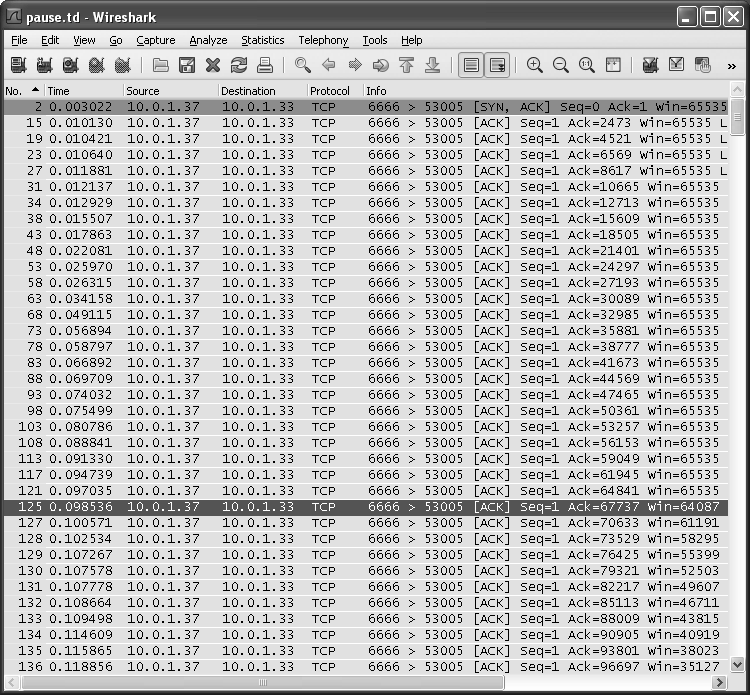
\includegraphics[width=0.7\textwidth]{imgs/15/15-11.png}
	\caption{比较相似环境下使用 Nagle算法与否的延}
\end{figure}
从图15-11 中可以看到,在接收了100多个包后,窗口大小仍然维持在64KB。这是由于自动窗口调节算法(参见 15.5.4节)默认分配了 TCP 接收端的缓存。然而,随着可用缓存
的减少,可以看到在125号包之后,窗口开始减小。随着大量的ACK 到达,窗口进一步减小,每个到达的ACK 号都增大2896字节。这表明接收端在存储这些数据,但应用程序并没
有处理。如果我们进一步观察,会发现最终接收端已经没有更多空间来存储到达的数据(见图 15-12)。

从图15-12 中可以看到,151号包耗尽了 327字节大小的窗口,Wireshark 显示“TCP窗口满”(TCP Window Full)。约200ms后,在4.979s时刻,零窗口通告产生,表明无法接
收新的数据。窗口最后的可用空间已满,接收端应用程序暂停处理数据,直到20.143s时刻。

收到零窗口通告后,发送端每隔5s共发送了三次窗口探测以查看窗口是否打开。在20s时刻,接收端开始处理 TCP 队列中的数据。因此有两个窗口更新传送至发送端,表明可以
继续传输数据(64KB)。窗口更新并不是对新数据的确认,而只是将的日右边界有弦。这时,发送端可以恢复正常的数据传输。

随着接收端可用缓存的逐渐减小,在一段时间后,窗口开始减小。如果接收端应用程序一直不处理任何数据,且发送端持续发送,窗口最终会缩减为0
\begin{figure}[!htb]
    \centering
	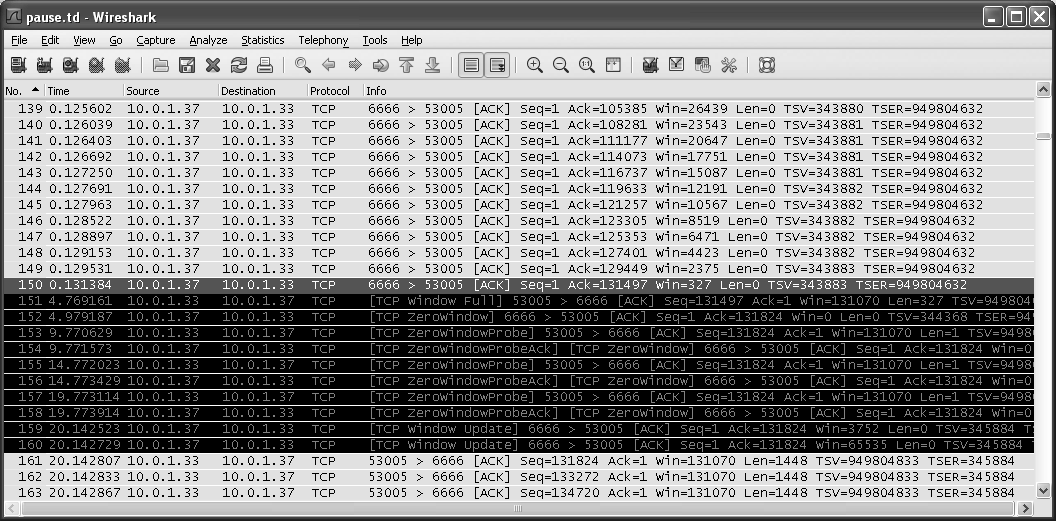
\includegraphics[width=0.7\textwidth]{imgs/15/15-12.png}
	\caption{接收端缓存已满。当接收应用程序再次开始处理数据时,窗口更新会通知发送端可继续发送}
\end{figure}

从图15-11 和图15-12中可以总结出以下几点:
\begin{enumerate}
    \item 发送端不必传输整个窗口大小的数据。
    \item 接收到返回的 ACK 的同时可将窗口右移。这是由于通告窗口是和该报文段中的ACK号相关的。
    \item 窗口大小可能减小,如图15-11所示,但窗口右边界不会左移,以此避免窗口收缩。
    \item 接收端不必等到窗口满才发送 ACK。
\end{enumerate}

此外,还可通过观察吞吐量随时间的变化函数得到一些启发。使用 Wireshark的“统计|TCP 流图|吞吐量图”(Statistics | TCP Stream Graph | Throughput Graph) 功能,可以得到图
15-13 所示的时间序列。
\begin{figure}[!htb]
    \centering
	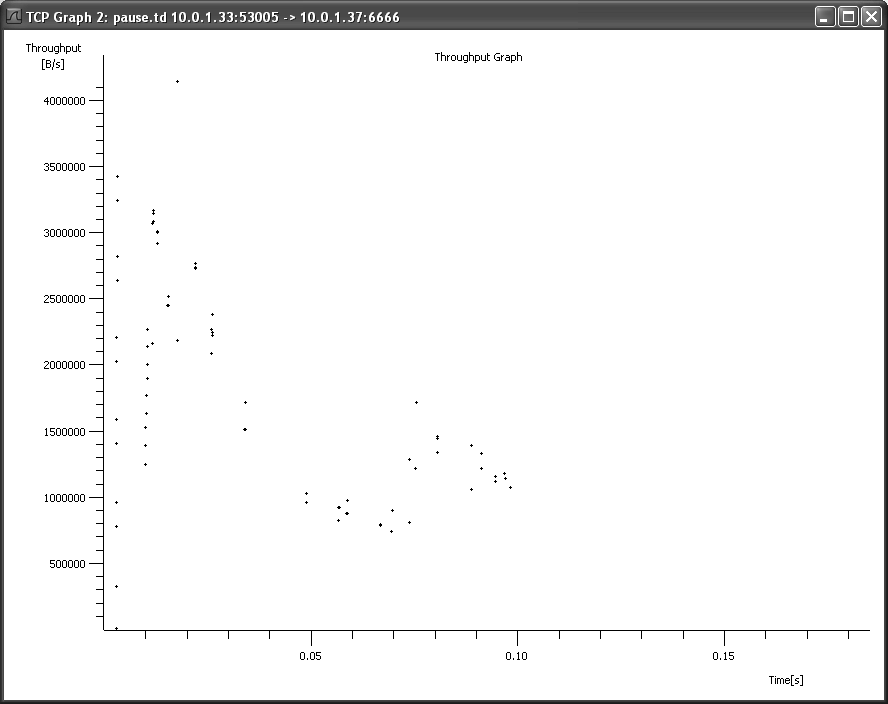
\includegraphics[width=0.7\textwidth]{imgs/15/15-13.png}
	\caption{使用相对较大的接收缓存,即使在接收端应用处理数据前也能传输大量的数据}
\end{figure}

这里我们看到一个有趣的现象。即使在接收端处理任何数据前,连接依然能达到约1.3MB/s的吞吐量。这种状况一直持续到约0.10s时刻。之后,直到接收端开始处理数据前
(在20s时刻后),吞吐量基本上都为0。

\subsection{糊涂窗口综合征}
基于窗口的流量控制机制,尤其是不使用大小固定的报文段的情况(如 TCP),可能会出现称为糊涂窗口综合征(Silly Window Syndrome,sws)的缺陷。当出现该同题时,交换
数据段大小不是全长的而是一些较小的数据段\href{https://www.rfc-editor.org/rfc/rfc0813}{[RFC0813]}。由于每个报文段中有用数据相对于头部信息的比例较小,因此耗费的资源也更多,相应的传输效率也更低。

TCP 连接的两端都可能导致SWS 的出现:接收端的通告窗口较小(沒有等到窗口变大才通告),或者发送端发送的数据段较小(没有等待将其他数据组合成一个更大的报文段)。
要避免 SWS 问题,必须在发送端或接收端实现相关规则。TCP 无法提前预知某一端的行为。需要遵循以下规则:
\begin{itemize}
    \item 对于接收端来说,不应通告小的窗口值。\href{https://www.rfc-editor.org/rfc/rfc1122}{[RFC1122]}描述的接收算法中,在窗口可增至一个全长的报文段(即接收端 MSS)或者接收端缓存空间的一半(取两者中较小者)之前,不能通告比当前窗口(可能为0)更大的窗口值。注意到可能有两种情况会用到该规则:当应用程序处理接收到的数据后使得可用缓存增大,以及 TCP接收端需要强制返回对窗口探测的响应。
    \item 对于发送端来说,不应发送小的报文段,而且需由Nagle 算法控制何时发送。为避免SWS 问题,只有至少满足以下条件之一时才能传输报文段:
    \begin{itemize}
        \item 全长(发送 MSS 字节)的报文段可以发送。
        \item 数据段长度>=接收端通告过的最大窗口值的一半的,可以发送。
        \item 满足以下任一条件的都可以发送:(i)某一ACK 不是目前期盼的(即没有未经确认的在传数据);(ii)该连接禁用 Nagle 算法。
    \end{itemize}
\end{itemize}

条件(a)最直接地避免了高耗费的报文段传输问题。条件(b)针对通告窗口值较小,可能小于要传输的报文段的情况。条件(c)防止TCP 在数据需要被确认以及 Nagle 算法启
用的情况下发送小报文段。若发送端应用在执行某些较小的写操作(如小于报文段大小),条件(c)可以有效避免SWS。

上述三个条件也让我们回答了以下问题:当有未经确认的在传数据时,若使用Nagle 算法阻止发送小的报文段,究竟多小才算小?从条件(a)可以看出,“小”意味着字节数要小
于 SMSS(即不超过 PMTU 或接收端MSS 的最大包大小)。条件(b)只用于比较旧的原始主机,或者因接收端缓存有限而使用较小通告窗口时。

条件(b)要求发送端记录接收端通告窗口的最大值。发送端以此猜测接收端缓存大小。尽管当连接建立时缓存大小可能减小,但实际这种情况很少见。另外,前面也提到过,TCP
需要避免窗口收缩。

\subsubsection{例子}
下面我们通过一个具体的例子来观察SWS避免的行;本例也包含持久计时器。这里使用我们的sock 程序,发送端主机为 Windows XP 系统,接收端为 FreeBSD,执行三次
2048字节的写操作传输。发送端命令如下:
\begin{verbatim}
    C:\> sock -1 -n 3 -W 2048 10.0.0.8 6666
\end{verbatim}
接收端相应的命令为:
\begin{verbatim}
    FreeBSD& sock -i -s -P 15 -p 2
-× 256
-R 3000 6666
\end{verbatim}

该命令将接收端缓存设为3000字节,在首次读数据前有15s的初始延时,之后每次读都会引入2s的延时,每次读的数据量为256字节。设置初始延时是为使接收端缓存占满,
最终迫使传输停止。这时通过使接收端执行小的读操作,我们期望看到它执行SWS避免。利用 Wireshark 可以得到如图15-14所示的记录。

整个连接的传输内容如图所示。包长度是根据每个报文段中携带的 TCP 有效载荷数据描述的。在连接建立过程中,接收端通告窗口为3000字节,MSS为1460字节。发送端在
0.052s时刻发送了一个 1460字节的包(包4),在0.053s时刻发送了588字节的包(包5)。两者总和为 2048字节,为应用写操作的大小。包6是对这两个包的确认,并提供了一个952
字节的窗口通告(3000-1460-588=952)。
\begin{figure}[!htb]
    \centering
	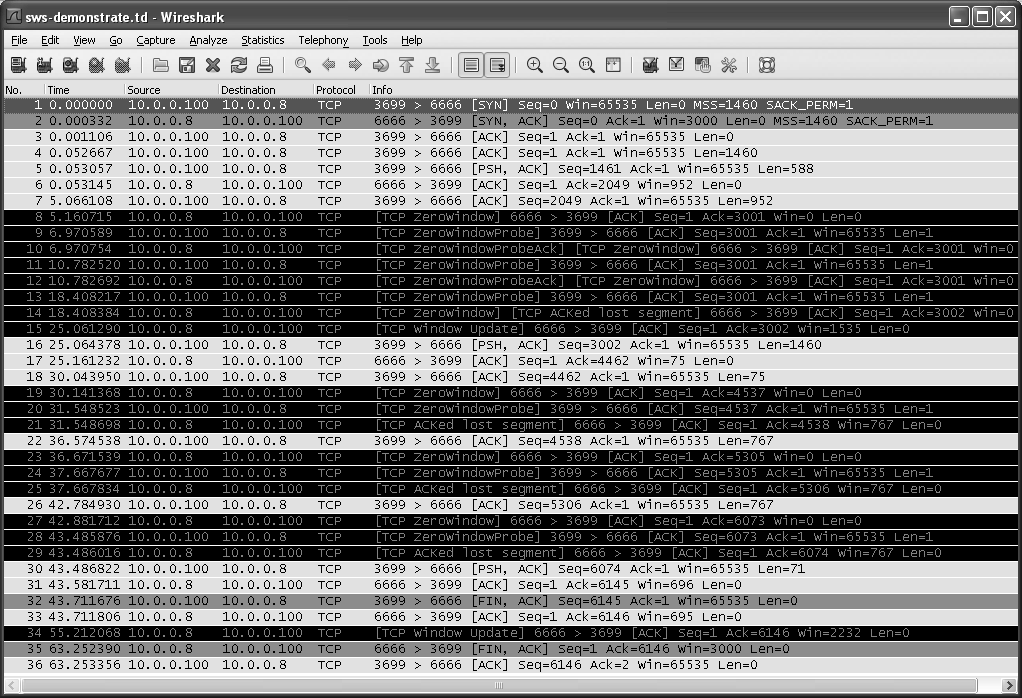
\includegraphics[width=0.7\textwidth]{imgs/15/15-14.png}
	\caption{SWS避免的行为分析。由于在0.0538时刻执行SWS 避免,发送端没有使用通告窗口传输数据。相反,一直等到5.066s 时刻,同时也有效地执行了窗口探测。通过14号包可以看到接收端SWS避免,即使已经处理了部分数据,接收端依然通告零窗口}
\end{figure}

952 字节的窗口(包6)并没有一个 MSS大,所以Nagle 算法阻止了发送端的立即发送。相反,发送端等待了 5S,直到特续计时器超时,才发送了一个窗口探测。考虑到无论如
何都要发送一个包,因此发送端发送了允许的952 字节数据填满了可用窗口,因此包8返回了零窗口通告。

下一个事件发生在6.970s时刻,TCP发送了一个窗口探测,即在接收到首个零窗口通告约25后。探测包本身包含一个字节的数据,图中 Wireshark显示为“TCP Zero WindowProbe",
但对该探测包的 ACK 号却没有增大(Wireshark 将其标记力“TCP Zero WindowProbeAck”),因此这一个字节的数据并没有被接收端保存。在10.7828时刻又产生了一个探测包(约45后),
接着 18.408s 时刻又产生一个(约8s以后),表明其发送间隔随时间呈指数增长。注意到最后一次窗口探测中包含的一个字节的数据已被接收端确认。

在25.061s时刻,在上层应用执行了6次256字节的读数据操作后(每次同隔25),窗口更新表明现在接收端缓存中有 1535字节(ACK 号加1)的可用空间。根据接收端SWS避
免规则,该数位已“足够大”。发送端开始继续传送数据。在25:0645 时刻发送了1400字节的包,在25.161s 时刻得到了对 4462 字节数据的 ACK,这时通告窗口大小只有75字节(包
17)。该通告似乎违背了我们之前的规则,即窗口值应至少为一个 MSS(对FreeBSD 来说)或总级存空间的四分之一。出现这种情况的原因在于避免窗曰收缩。最后一个窗口更新中
(包15),接收端通告窗口右边界为(3002+ 1535)-4537。如果当前ACK(包17)通告的窗日小于75字节,像接收端SWS 避免要求的那样,窗口右边界就会左移,TCP是不允许出现
这种情况的。因此这 75字节的通告窗口代表一种更高的优先级:避免窗口收缩优先于避免SWS。

通过包17和包18之间的5s的延时,我们再次看到发送端的SWS避免。发送端被强制要求发送一个75字节的包,接收端返回一个零窗口通告响应。在1s之后的包20是再次的
窗口探测,得到了767字节的可用窗口。又一轮的发送端SWS避免导致了Ss的延时;发送端填满窗口后,再次返回零窗口通告;这种状况一直重复。最终发送端没有新的数据发送而
终止。包30代表发送的最后一个包,在20s后连接终止(由于接收端应用每次读数据的间隔为2s)。

为了理解上层应用行为、通告窗口和SWS避免之间的关系,我们将连接的动态传输以表格的形式展现出来。表15-1 给出了发送端和接收端的行为,以及接收端应用执行读操作
的估计时间。

SWS 避免的通告窗口及应用层动态变化情况


在表15-1中,第1列表示图中出现的每个传输行为的相对时刻,带三位小数的数值是Wireshark 显示的时间值(参见图15-14)。而不带小数的则是接收端主机行为的估计时刻,
图中并没有显示。

接收端缓存中的数据(表中标记为“已存数据”)随着新数据的到达而增加,随着上层应用的读取而减少。我们想了解的是接收端返回给发送端的窗口通告中包含的内容。这样就
能知道接收端是怎样避免SWS的。

如前所述,第一次SWS避免是包6和包7之间的5s延时,由于窗口大小只有952字节,发送端一直避免传输直到被强制要求发送数据。传输完成后,接收端缓存满,之后产生
了一系列的零窗口通告和窗口探测交换。我们可以看到持续计时器指示的时间间隔星指数增长:探测包的发送时刻为6.970s,10.782s和18.408S。这些时刻与发送端首次接收到零窗口
通告的时刻5.160s 的间隔约为2S、4s、8S。

尽管上层应用在15s和17s时刻读数据,但至18.408s时刻为止只读了512字节。根据接收端SWS 避免规则要求,由于512字节的可用缓存既小于总缓存空间(3000字节)的一
半,也没有达到一个 MSS(1460字节),因此不能提供窗口更新。发送端在 18.408s时刻发送了一个窗口探测(报文段13)。该探测包被接收,由于缓存有一定的可用空间,因此其中
包含的一个字节数据也被保存,报文段12和14之间的ACK号的增长验证了这一点。

尽管有511字节的可用空间,但接收端再次实施了SWS 避免。接收端 FreeBSD 在实现sWS避免时区分了何时发送窗口更新与怎样响应窗口探测。它遵循\href{https://www.rfc-editor.org/rfc/rfc1122}{[RFC1122]} 中的规则,
只在通告窗口至少为总接收缓存的一半(或一个 MSS)时才发送窗口更新,并且只有当窗口至少为一个 MSS 或超过总接收缓存的四分之一才响应窗口探测。但在这里,511字节小于一
个 MSS 且不到3000/4=750字节,因此接收端只好对报文段13的ACK 中包含的通告窗口设为0。

直到25 时刻为止,上层应用完成了6次读操作,接收端缓存有 1535字节空闲(大于总的3000字节的一半),因此发送了一个窗口更新(报文段15)。发送的数据为全长报文段
(报文段16),接收到的ACK 中包含的通告窗口仅为75字节。在接下来的5S内,两端都执行SWS 避免。发送端需要等待一个更大的通告窗口,上层应用在27s时刻和 29s时刻执行
读操作,但只有587 字节的空间,不足以发送窗口更新。因此,发送端持续等待了 Ss并最终发送了剩余的75字节,迫使接收端再次进入SWS避免状态。

接收端没有提供窗口更新,直到31.548s时刻发送端的持续计时器超时,发送了一个窗口探测。接收端响应了一个非零窗口,为767 字节(大于总接收级存的四分之一)。该窗口值
对发送端并非足够大,因此继续执行发送端的SWS 避免。发送端等待了SS,之后一直重复上述过程。最终,在43.486s 时刻,最后的71字节发送完并得到确认。该 ACK 中包含696字节
的窗口通告。尽管小于总接收缓存的四分之一,为了避免窗口收缩,通告窗口并没有设为0。

从报文段32开始,不再包含数据,连接开始关闭。随即得到的确认中窗口大小为695字节(接收端的FIN消耗了一个序列号)。在上层应用再次完成6次读操作后,接收端提供
了一个窗口更新,但发送端已经完成所有数据的发送,并保持空闲状态。上层应用又执行了4次读操作,其中3次返回256字节,最后1次没有返回,表明已经无数据到达。此时,接
收端关闭连接并发送 FIN。发送端返回了最后一个 ACK,双向连接结束。

由于发送端应用在执行3次2048字节的写操作后开始关闭连接,在发送完报文段32后,发送端从 ESTABLISHED 状态变为 \verb|FIN_WAIT_1| 状态(参见第13章)。接着在接收到报
文段33后,进入\verb|FIN_WAIT_2|状态。尽管在这时接收到了窗口更新,但发送端没有任何动作,因为它已经发送了 FIN并经确认(这一阶段没有计时器)。相反,在接收到对方的FIN
前,它只是静静等待。这就是我们没有看到更多的传输直至接收到FIN 的原因(报文段35)。

\subsection{大容量缓存与自动调优}
从前面的章节可以看到,在相似的环塊下,使用较小接收缓存的 TCP 应用的吞吐性能更差。即使接收端指定一个足够大的级存,发送端也可能指定一个很小的缓存,最终导致性
能变差。这个问题非常严重,因此很多 TCP 协议栈中上层应用不能指定接收缓存大小。在多数情况下,上层应用指定的级存会被忽视,而由操作系统来指定一个较大的固定值或者动
态变化的计算值。

在较新的 Windows版本(Vista/7)和Linux 中,支持接收窗口自动调优[S98]。有了自动调优,该连接的在传数据值(连接的带宽延时积———个重要概念,将在第16章讨论)需
要不断被估算,通告窗口值不能小于这个值(假如剩余缓存空间足够)。这种方法使得TCP达到其最大可用吞吐率(受限于网络可用容量),而不必提前在发送端或接收端设置过大的级
存。在 Windows 系统中,默认自动设置接收端缓存大小。然而,也可以通过 netsh 命令更改默认值:
\begin{verbatim}
    C: \> netsh interface tcp
set heuristics disabled
C:\> netsh interface tcp set global autotuningleve1=x
\end{verbatim}

这里X可设置力 disabled、highlyrestricted、restricted、normal 或 experimental。不同的设置值会影响接收端通告窗口的自动选择。在disabled 状态下,禁用自动调优,窗口大小使
用默认值。restricted 模式限制窗口增长,normal 允许其相对快速增长。而 experimental 模式允许窗口积极增长,但通常并不推荐normal模式,因为许多因特网站点及某些防火墻会干
扰,或没有很好地实现 TCP 窗口缩放(Window Scale)选项。

对于 Linux 2.4及以后的版本,支持发送端自动调优。2.6.7及之后的版本,两端都支持该功能。然而,自动调优受制于缓存大小。下面的 Linux sysctl 变量控制发送端和接收端的
最大缓存。等号之后的值为默认值(根据不同的Linux 版本可能会有不同),如果系统用于高带宽延时积的环境下,上述值需要增大。

\begin{verbatim}
    net.core.rmem_max = 131071
net.core.wmem_max = 131071
net.core.rmem_default = 110592
net.core.wmem_default = 110592
\end{verbatim}

另外,通过下面的变量设定自动调优参数:
\begin{verbatim}
    net. ipv4.tep_rmem = 4096 87380 174760
net.ipv4.tcp_wmem = 4096 16384
131072
\end{verbatim}

每个变量包含三个值:自动调优使用的缓存的最小值、默认值和最大值。
\subsubsection{例子}
为演示接收端自动调优行为,这里采用Windows XP 发送端(设为使用大容量窗口和窗口缩放)和Linux 2.6.11 接收端(支持自动调优)。在发送端运行如下命令:
\begin{verbatim}
    C:\> gock -n 512 -1 10.0.0.1 6666
\end{verbatim}

对接收端,我们不对接收级存做任何设置,但在上层应用读取数据前设置20s的初始延时:
\begin{verbatim}
    Linux8 sock -1 -g -v -p 20 6666
\end{verbatim}

为描述接收端通告窗口的增长,可以利用Wireshark 来显示包传输情况,并根据接收端地址来进行分类(参见图15-15)。在连接建立阶段,接收端初始窗口值为1460字节,初始
MSS 为1412字节。由于其采用了窗口缩放,会有2倍的变动(图中没有显示),使得最大可用窗口为256KB。可以看到在完成第一个包传输后,窗口有了增长,相应地发送端也提高了
发送速率。在第16章中我们将会讨论 TCP拥塞控制的发送速率。现在,我们只需要知道发送端何时开始发送,通常情况下其首先发送一个包,接着每收到一个ACK,发包数就增加
一个 MSS。因此,每接收一个 ACK,就会发送两个包(每个包长度为一个 MSS)。
\begin{figure}[!htb]
    \centering
	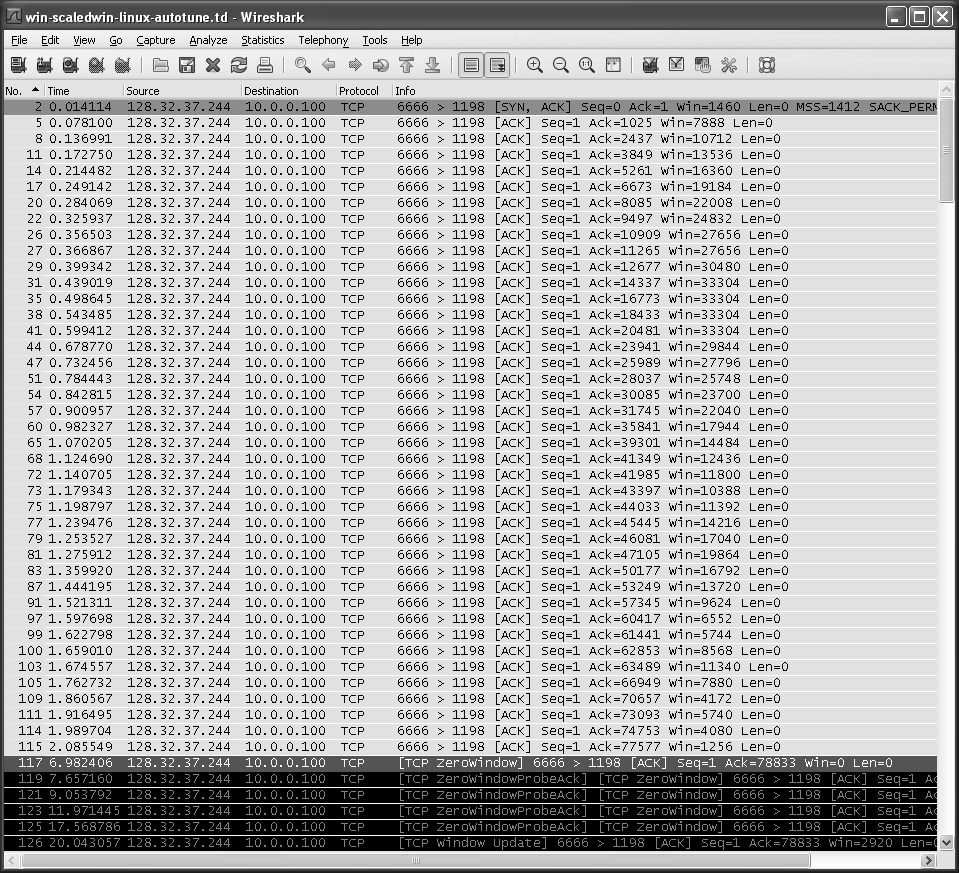
\includegraphics[width=0.7\textwidth]{imgs/15/15-15.png}
	\caption{Linux 接收端执行自动调优,窗口值随着接收数据的增多而增大。由于上层应用在20s之内都没有读取数据,最终窗口将关闭}
\end{figure}

观察窗口通告值 10712、13536、16360、19184 可以发现,每接收一个ACK,窗口就增长两个 MSS,这与发送端拥塞控制操作相一致(第16 章会讨论)。假设接收端存储空
间足够大,根据拥塞控制局限性,通告窗口总是大于允许发送的数据量。这种方式是最优的一-在保持发送端最大发送速率的情况下,接收端通告和使用的缓存空间最小。

当接收端缓存资源耗尽时,自动调优也会受影响。在本例中,0.678s时刻窗口达到最大值33304字节,接着开始减小。这是由于上层应用停止读取数据,导致缓存被占满。当20s
后上层应用继续读操作时,窗口再次增大,并超过了之前的最大值(参见图15-16)。
\begin{figure}[!htb]
    \centering
	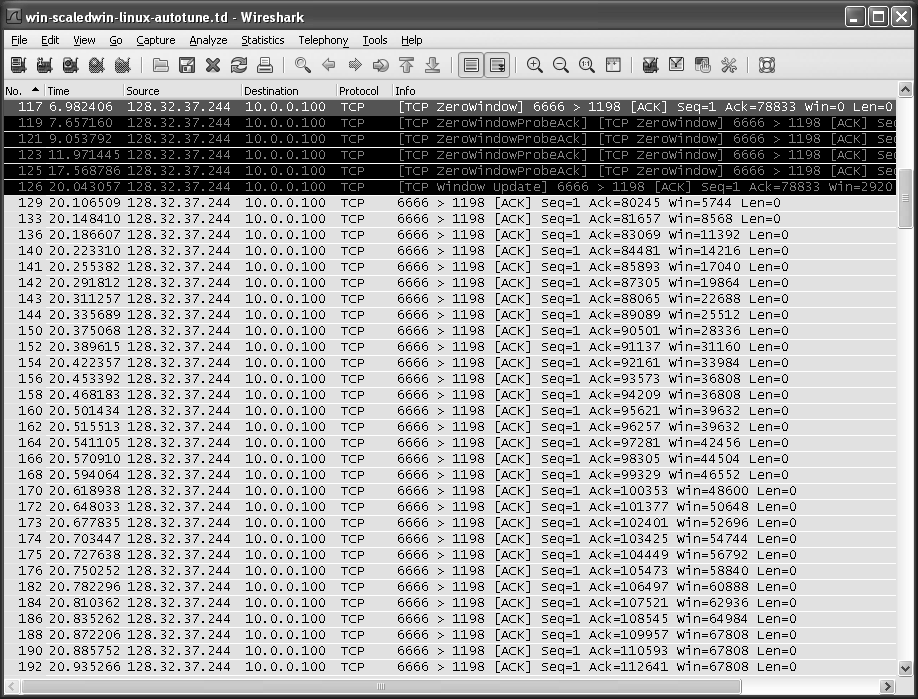
\includegraphics[width=0.7\textwidth]{imgs/15/15-16.png}
	\caption{当上层应用暂停读取数据时,接收端缓冲区开始被占满,自动调优也相应停止。随着读操作的继续执行,通告窗口也逐渐增大,并超过了之前的最大值}
\end{figure}

零窗口通告(包 117)使得发送端执行了一系列的窗口探测,但返回的仍是一系列的零窗口。在 20.043s时刻恢复读数据操作时,发送端接收到了窗口更新。每接收到一个ACK,
窗口就增大两个 MSS。随着数据的发送、接收和处理,通告窗口达到了最大值67808。该版本的Linux 也测量相邻两次读操作完成的时间,并与估计 RTT值相比较。如果 RTT 估计值
增大,那么缓存也将增大(但不会因 RTT 的减小而减小缓存)。这样即使在连接的带宽延时积增大的情况下,自动调优也保持接收端通告窗口优先于发送端窗口。

随着广域网络连接速度的增长,TCP 应用使用的缓存太小已成为严重局限。在美国,全国范围内的RTT约为 100ms,在一个1Gb/s的网络中使用64KB的窗口将 TCP 吞吐量限制
在约640KB/s,而计算的最大值可以达到约130MB/s(99\%的带宽都浪费了)。实际上,如果在相同网络环境下使用较大容量的缓存,吞吐性能将提升100倍。Web100工程[W100]应
得到更多关注和信心。它开发了一系列工具和改进软件,致力于使应用从众多的TCP 实现中获得最优的吞吐性能。

\section{紧急机制}
我们在第12章中已经提到,TCP头部有一个位字段URG用来指示“紧急数据”。应用在执行写操作时,可通过设置 Berkeley 套接字 API(\verb|MSG_00B|)的特殊选项将数据标记
为紧急,但\href{https://www.rfc-editor.org/rfc/rfc6093}{[RFC6093]}不再推荐设置紧急数据。当发送端 TCP收到这类写操作要求时,会进入称为紧急模式(urgent mode)的特殊状态。它记录紧急数据的最后一个字节,用于设
置紧急指针(Urgent Pointer)字段,随后发送端生成的每个 TCP头部都包含该字段,直到应用停止紧急数据写操作,并且所有序列号在紧急指针之前的数据都经接收端确认。根据
\href{https://www.rfc-editor.org/rfc/rfc6093}{[RFC6093]},紧急指针指示的是紧急数据之后的一个字节。大量的 RFC文档中对紧急指针的阐述都存在语义上的模糊和二义性。对于使用IPv6 的超长数据报而言,紧急指针值需设为
65535,用于指示紧急数据的末端位于 TCP数据域的最后\href{https://www.rfc-editor.org/rfc/rfc2675}{[RFC2675]},如果使用传统的16位紧急指针字段就不能表示 64KB的偏移。

当收到UGR 置位的报文段时,TCP 接收端就会进入紧急模式。接收端应用可以调用标准套接字 API (select O)来判断是否进入紧急模式。紧急机制会带来操作上的混淆,因为
Beikeley 套接字 API 和文档中用到了术语:带外(Out-Of-Band, 0OB)数据。而实际上TCP并没有实现任何OOB 功能。相反,差不多所有 TCP实现在将紧急数据的最后一个字节传输
给上层应用时,在接收端使用了一个截然不同的API 参数。接收端必须要设置 \verb|MSG_OOB|选项检索该字节,或者设置 \verb|MSG_OOBINLINE| 使该字节保持在正常数据流传输(在使用紧
急机制情况下,需要用到该方法)。

\subsection{例子}
为更好地理解紧急机制,我们通过一个例子来具体观察紧急模式的行为,包括在零窗口事件期间发生的状况。这里使用 Mac OS X 发送端和Linux 接收端。为获得零窗口,我们首
先在接收端限制接收窗口自动调优:

\begin{verbatim}
    Linux# sysctl -w net. ipv4.tcp_rmem='4096 4096 174760'
    Linux& sock -1 -v -B -D 1 -P 10 5555
\end{verbatim}

第一个命令确保接收窗口的自动调整幅度不超过4KB,这样就可以清楚地看到窗口关闭时发生的情形。第二个命令使服务器在读数据前等待 10s,并在每次读操作间等待1s。在客
户端我们执行如下命令:
\begin{verbatim}
    Mac& sock -1 -n 7 -0 7 -D1 -8 8192 10.0.1.1
SO_SNDBUF
5555
- 8192
connected on 10.0.1.33.51101 to 10.0.1.1.5555
TCP_MAXSEG = 1448
wrote 1024 bytes wrote 1024 bytes wrote 1024 bytes wrote 1024 bytes wrote 1024 bytes wrote 1024 bytes
wrote 1 byte of urgent data
wrote 1024 bytes
\end{verbatim}

该命令使得客户端每隔1s执行一次写操作,共7次,每次1024字节,且在最后一次写之前写了1个字节的紧急数据。客户端级存设置为 8192 字节,由于在TCP 发送数据前所有
数据都暂时存储在发送端,因此缓存已足够大,该应用可立即得到执行。

如图 15-17所示,接收端初始通告窗口右边界为 2800,并很快增至5121。在1.0s时刻,应用执行了一次写操作,窗口有边界前进至6145。之后由于自动调优在高于4192 字节时被
禁用且接收应用没有执行读操作,窗口没有继续增长。直到10.0s时刻,发送端执行了窗口探测,但依旧没有获得窗口增长。最终在 10.0s 时刻之后,接收端开始继续读取数据,窗口
打开,发送端继续发送直至完成传输。包交换情况如图15-18所示。
% \begin{figure}[!htb]
%     \centering
% 	\includegraphics[width=0.7\textwidth]{imgs/15/15-17.png}
% 	\caption{在执行6次写操作后,接收端窗口没有前移。TCP发送端暂停发送,直至在10s时刻窗口打开}
% \end{figure}

紧急模式的“出口点”定义为TCP报文段中序列号字段与紧急指针字段之和。每个TCP 连接只维护一个紧急“点”(序列号偏秘),因此紧急指针字段为空的包会导致前面的紧
急指针包含的信息丢失。报文段16为第一个包含有效紧急指针的报文段,使得序列号 6146到达出口点。注意到该序列号可能并不在指示的报文段中,而可能在之后的报文段中。例如
报文段17就是这种情况,它没有包含任何数据,只有紧急指针(值为1)。

如前所述,有个问题一直存在争议,即出口点指示的是紧急数据的最后一个字节还是非紧急数据的第一个字节。TRFCI122]认为指针指示的是紧急数据的最后一个字节。然而,基
本上所有的TCP实现都没有遵循该规定,因此\href{https://www.rfc-editor.org/rfc/rfc6093}{[RFC6093]}认识到了这一问题,并修改规范让指针指向非紧急数据的第一个字节。在本例中,序列号为6145的字节包含工由sock 客户
瑞产生的】字节紧急数据,但在所有的报文段中,紧急指针的信为1,序列号为6145。因此,可以看出该 TCP 实现中(大多数 TCP 实现都如此),出口点为非紧急数据的第一个字节
的序列号。
\begin{figure}[!htb]
    \centering
	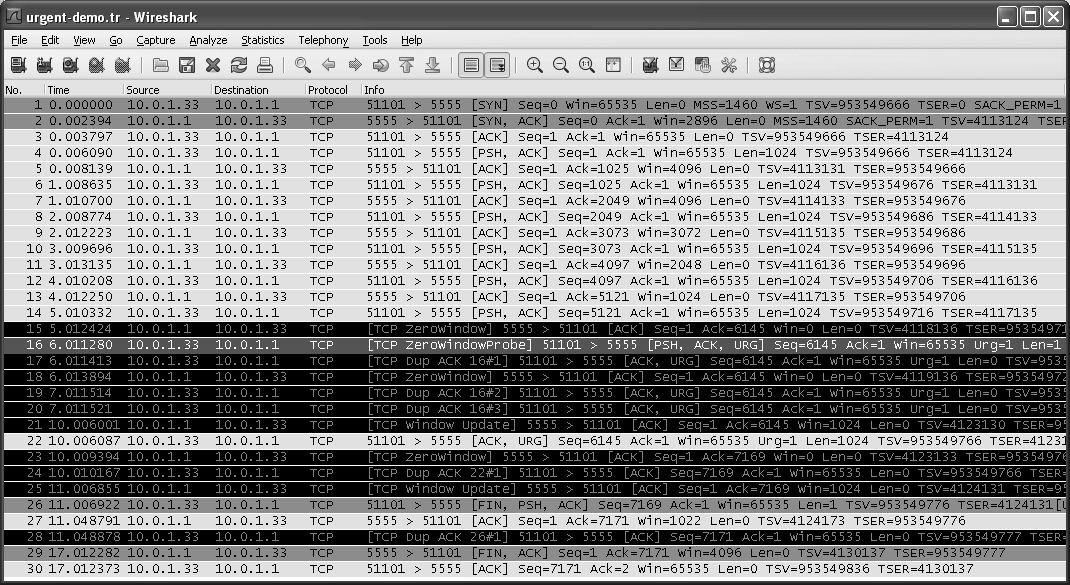
\includegraphics[width=0.7\textwidth]{imgs/15/15-18.png}
	\caption{整个数据传输在5.0125时刻出现了一次零窗口通告。当应用执行下一次写操作时,发送端TCP 进入紧急模式,6.0113s时刻发送的窗口探测报文段中的URG置位。
    在第7秒执行最后一次写操作并关闭,产生了两个空的报文段。10.006s时刻的窗口更新重新启动数据传输。10.009s时刻的零窗口通告使得传输再次停止,同时由于紧急指针已被确认,
    因此可以退出紧急模式。11.007s时刻的FIN 包含了数据的最后一个字节}
\end{figure}
从这个例子可以看到,TCP将紧急数据携带在数据流中传输(而非“带外传输”)。如果某个应用确实需要独立的信号通道,可以简单采用另一个 TCP 连接。(某些传输层协议确实
提供大多数人认为的OOB 数据,即像通常数据链路那样使用同一个连接,但有独立的逻辑数据路径。TCP 并不提供该功能。)


\section{与窗口管理相关的攻击}
TCP 窗口管理可能受到多种攻击,主要形式为资源耗尽。通告窗口较小会使得TCP传输减慢,因此会更长时间地占用资源,如存储空间。这一点已被用于针对传输性能较差的网
络攻击(即蠕虫)。例如,LaBrea tarpit程序[LO1]在完成 TCP 三次握手后,要么不做任何行为,要么只产生一些最小的应答,使得发送速率不断减慢。通过此法来保持发送端忙碌,本
质上是减慢蜗虫的传播速度。因此 tarpit 程序是针对流量攻击的一类攻击。

比较新的攻击发布于2009年[109],它基于已知的持续计时器的缺陷,采用客户端多“SYN cookies” 技术(参见第13章)。所有必要的连接状态都可以下载到受害主机进
行,从而使得攻击方主机消耗最少的资源。这种攻击本身类似于LaBrea 思想,只是其针对持续计时器。同一台服务器可能受到多个此类攻击,最终导致资源耗尽(如系统内存耗
尽)。[C723308] 提出了一种解决方法,即当推断出现资源耗尽时,允许其他进程关闭TCP连接。


\section{总结}

交互式数据传输的报文段通常小于SMSS。接收方收到这些分组时可能会采取延时确认的方法,希望能将这些 ACK与需要发送给对方的数据一起捎带传输。这种方法可以减少传
输报文段的数目,特别是在交互式流量传输中,服务器需要对客户端的每个按键都返回响应。然而,延时确认也会引人额外的延时。

对于RTT 相对较大的连接,如WAN,通常使用Nagle算法来减少较小报文段数目。该算法限制发送端在任意时刻发送单个小数据包。这样会减少较小数据包在网络连接中的
数目,从而减小传输资源开销,但同时也可能引人上层应用无法接受的延时。另外,延时ACK与Nagle算法的互相作用可能导致短暂的死锁。基于上述原因,有的应用可能禁用
Nagle算法,而大多数交互式应用都使用该功能。

TCP通过在其发送的每个 ACK 中包含一个窗口通告来实现流量控制。该窗口告诉对方自己还有多少缓存空间。当没有使用 TCP 窗口缩放选项时,最大通告窗口为65535字节。
否则最大窗口值可以更大(约1GB)。

通告窗口值可能为0,表明接收端缓存已满。这时发送端停止发送,并以一定间隔不断地发送窗口探测,发送间隔类似于超时重传(参见第14章),直到收到ACK 表明窗口变大,
或收到接收端主动发送的窗口通告(窗口更新)表明有可用缓存空间。这种以一定间隔连续发送的行 可能被用于资源耗尽攻击。

随着TCP 的不断发展,出现了一种奇怪的现象。当通告窗口较小时,发送端会立即发送数据填满该窗口,这样在连接中就会出现大量高耗费的小数据包。这种现象被称为“糊涂
窗口综合征”。针对这一问题,在 TCP发送端和接收端都有相应的策略。对发送端来说,若通告窗口较小则避免发送小数据包;接收端则尽量避免通告小窗口。

接收端窗口大小受限于其缓存大小。一般来说,如果上层应用没有设置其接收缓存大小,就会为其分配一个相对较小的空间,这样即使在高带宽的传输路径上,传输延时仍旧很
大,导致网络吞吐性能变差。在较新的操作系统中不会出现上述问题,采用自动调优的方法可以高效地自动分配缓存大小。
